%!TEX root = Zusammenfassung.tex

\section{Mathematische Grundlagen}
% ---------------------------------------------------------------------------------------------------------------------
\subsection{Ordnungen}
\begin{description}
	\item[(partielle) Ordnung] reflexiv, transitiv, antisymmetrisch
	\item[minimale, maximale Elemente] fehlende Existenz von kleineren, größeren Elementen
	% komponentenweise Ordnung
	\item[größtes, kleinstes Element] alle anderen sind kleiner, größer
	% Verband der Teilmengenrelation
	\item[totale Ordnung] beliebige zwei Elemente vergleichbar
	\item[Kette, Antikette] Menge von nur (un-)vergleichbaren Elementen, genauer:
		\[A \text{ Antikette } \Leftrightarrow (\forall x,y \, :\, x,y\in A \land x\not= y : \neg ((x\leq y) \lor  (y\leq x)))\]
	\item[maximale (Anti-) Kette] es gibt keine echte Obermenge, die eine \hbox{(Anti-)} Kette ist.
		\\Maximale Antiketten sind als Mengen partiell geordnet
	\item Theorem 1.1 in \cite{Ban93}.
	\item[lexikographische, komponentenweise Ordnung] sollten bekannt sein.
\end{description}

% ---------------------------------------------------------------------------------------------------------------------
\subsection{Graphen}

\begin{description}
	\item[(un)gerichtete Graphen] Knoten, Bögen/Kanten (mit/ohne Richtung)\\(Anm: wir verwenden ``Kanten'' auch im gerichteten)
	\item[Wege, Pfade] klar; Pfad beachtet die Richtung
	\item[Zyklen, Schleifen] Weg, Pfad mit Anfang = Ende
	\item[schwach zusammenhängend] ungeachtet der Richtung
	\item[stark zusammenhängend] mit Beachtung der Richtung von jedem zu jedem
	\item[$n$-fach zusammenhängend] nach dem Löschen von $n\!-\!1$ beliebigen Kanten immer noch zusammenhängend
	\item[schwache, starke Zusammenhangskomponenten] Teilgraphen, die schwach, stark zusammenhängend sind
	\item[azyklische Kondensation] pro starke Zusammenhangskomponente ein Knoten;\\die ``schwachen Kanten'' übernehmen
\end{description}

\subsubsection*{Beispielgraph:}
\begin{center}
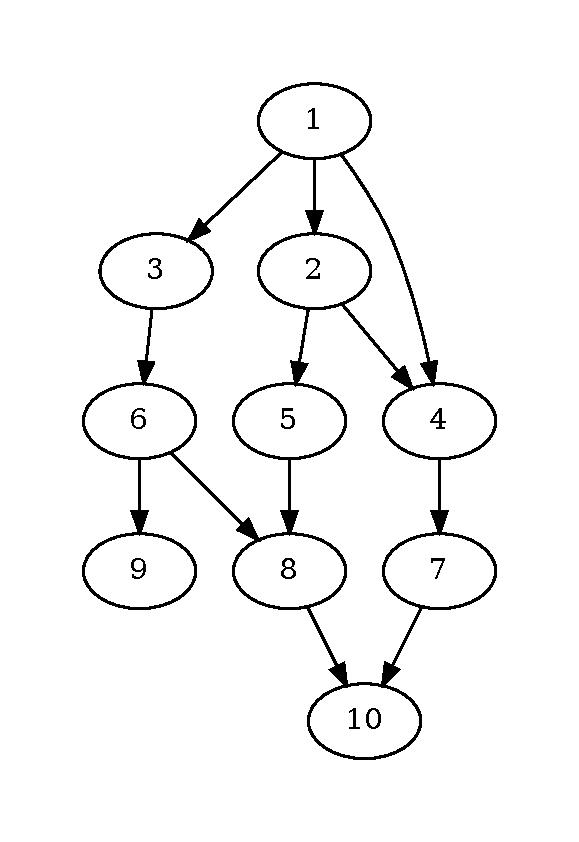
\includegraphics[scale=0.7]{images/BeispielgraphGraphentheorie.pdf}
\end{center}

\subsubsection{Bestimmung maximaler Ketten}
Von der $1$ an beginnend den Baum aufbauen, Knoten streichen wenn sie durch einen längeren
Pfad erreicht werden können. Tritt ein Knoten mehrfach mit gleicher Distanz zum Anfangsknoten
auf, bleiben beide Ketten bestehen. Sind alle Kanten ausgeschöpft, mit einem anderen Knoten von
vorne beginnen, der noch in keinem Baum aufgetaucht ist (Im Beispiel nicht der Fall).

Hier:
\[1 \rightarrow 3 \rightarrow 6 \rightarrow 9\]
\[1 \rightarrow 3 \rightarrow 6 \rightarrow 8 \rightarrow 10\]
\[1 \rightarrow 2 \rightarrow 5 \rightarrow 8 \rightarrow 10\]
\[1 \rightarrow 2 \rightarrow 4 \rightarrow 7 \rightarrow 10\]

\subsubsection{Bestimmung maximaler Antiketten}
Zunächst die transitive Hülle der Relation bestimmen. Das geschieht im Beispiel idealerweise
bei der 10 beginnend, da Kanten nur von kleineren zu größeren Zahlen existieren. Daraus können
die Antiketten der Länge 2 bestimmt werden. Diese lassen sich immer dann zu längeren Antiketten
verbinden, wenn $\{a,b\}, \{a,c\}, \{b, c\}$ Antiketten sind: Sie bilden zusammen $\{a,b,c\}$.
\textit{Maximale Antiketten} sind die mit der Länge $N$, wenn die längste Antikette $N$
Elemente hat.

Hier:
\[\{1\}, \{2,3\}, \{2,6\}, \{2,9\}, \{3, 4,5\}, \{3, 5, 7\}, \{4, 5, 6\}, \{4,5,9\}, \{4,8,9\},
\{5,6,7\},\{5,7,9\}, \{7,8,9\}, \{9,10\}\]

\subsubsection{Stark und schwach zusammenhängend}
\begin{description}
    \item[Schwach zusammenhängend] Graph zerfällt nicht in unzusammenhängende Teilgraphen.
    \item[Stark zusammenhängend] Jeder Knoten im Graph ist von jedem anderen aus erreichbar.
    \item[$n$-fach zusammenhängend] nach dem Löschen von $n−1$ beliebigen Kanten immer noch zusammenhängend
    \item[schwache/starke Zusammenhangskomponenten] Teilgraphen, die schwach/stark zusammenhängend sind
    \item[azyklische Kondensation] pro starke Zusammenhangskomponente ein Knoten; nur die ``schwachen Kanten'' übernehmen
\end{description}

% ---------------------------------------------------------------------------------------------------------------------
\subsection{Matrixalgebra}

\subsubsection{unimodulare Abbildungen}
\begin{enumerate}
	\item ganzzahlig; Determinante=$\pm$1; Inverses ganzzahlig
	\item Bilder von Polytopen unter unimodularen Abbildungen
	\item elementare Zeilentransformationen sind unimodulare Abbildungen:
		\begin{description}
			\item[Reversal] Multiplikation einer Zeile mit -1 (!)
			\item[Interchange] Vertauschen zweier Zeilen
			\item[Skewing] ein Vielfaches einer Zeile zu einer anderen addieren
		\end{description}
	\item Unimodularität abgeschlossen unter Multiplikation
	\item Wesentliches Verfahren: Zeilen-Stufen-Reduktion (Echelon Reduktion) einer Matrix $A$ durch eine unimodulare Transformation $U$: $U*A = S$
	\item Möglichkeit: Diagonalisierung durch anschließende elementare Spaltenoperationen $V$: $S*V = D$
	% \item keine Permutationsmatrizen
\end{enumerate}

\subsubsection{ganzzahlig-lineare Gleichungssysteme}
\begin{enumerate}
	\item ``normale'' Gauß-Elimination liefert alle rationalen Lösungen
	\item Einsetzen der frei wählbaren Variablen führt i.A. zu Brüchen in den nicht frei wählbaren Variablen
	\item Nachbearbeitung der freien Variablen ist möglich (um ganzzahlige Lösungen zu erhalten).
		Frage: gibt es eine direktere Berechnung?
	\item Bekannt: eine ganzzahlig-lineare Gleichung ist lösbar gdw. der ggT $g$ der Koeffizienten $a$ die rechte Seite $c$ teilt
	\item ggT$(a)$ steht in der Zeilen-Stufen-Form des Spaltenvektors $(a)$ oben; erste Zeile von $U$ liefert die Multiplikatoren für $a$
	\item Idee: ggT-Restriktion als erstes einsetzen um die Brüche zu vermeiden,
		die bei der Rückwärtssubstitution \`a la Gauß bei der letzten Substitution entstehen.
		Löungsmöglichkeiten: Spalten-Stufen-Form (ungewohnt) oder ``transponierte Darstellung''.
		Daher ab sofort:
	\item Variablenvektor $x$ von links multiplizieren (damit Matrizen transponiert) und Zeilen-Stufen-Transformation.
		Also: $x*A = c$. Dann gilt für eine einzelne Gleichung $x*a=c$ nach unimodularer Zeilen-Stufen-Transformation des Spaltenvektors $a$:
	\item Menge aller Lösungen: $(x_1,\cdots,x_m) = (c/g,t_2,\cdots,t_m)* U$
	\item Verallgemeinerung: $x*A = c$ lösbar gdw. $\exists t: t*S = c$. Menge aller Lösungen: $x = t*U$.
	% \item keine 2 Variables mit \psi_- und \psi_+
\end{enumerate}

\textbf{Beispiel}\\
Ziel: Eine ganzzahlige Lösung ist gewünscht \\
Erinnerung: $U*A = S$ und $x = t*U$

Gleichungssystem:
\begin{align*}
  4x_1 +  6x_2         & = 8 \\
  15x_1 + 21x_2 + 6x_3 & = 9
\end{align*}

Lösung nach Algorithmus:
\[\left(
\begin{array}{cc|ccc}
  4 & 15 & 1 & 0 & 0    \\
  6 & 21 & 0 & 1 & 0    \\
  0 & 6  & 0 & 0 & 1%
\end{array}%
\right) \leadsto \left(
\begin{array}{cc|ccc}
  2 & 6 & -1 & 1  & 0    \\
  0 & 3 & 3  & -2 & 0    \\
  0 & 0 & -6 & 4  & 1%
\end{array}%
\right)\]

Somit:
\[\left(
t_1, t_2, t_3
\right) *
\left(
\begin{array}{cc}
  2 & 6    \\
  0 & 3    \\
  0 & 0%
\end{array}
\right)
=
\left(
\begin{array}{cc}
  8 & 9
\end{array}
\right)\]

\[\Rightarrow t_1 = 4 \text{, } t_2 = \frac{(9-6*4)}{3} = -5 \text{, } \text{, }t_3 \in \mathbb{Z}\]

\[\left(
\begin{array}{c|cc}
  4 & 1 & 0    \\
  6 & 0 & 1%
\end{array}
\right) \leadsto \left(
\begin{array}{c|cc}
  2 & -1 & 1     \\
  0 & 3  & -2%
\end{array}
\right)\]

Damit ergibt sich als ggT die 2 und als Lösung des Ursprungssystems:

\[x = (x_1, x_2, x_3) = t * U =
(4,-5,t_3) *
\left(
\begin{array}{ccc}
  -1 & 1  & 0 \\
  3  & -2 & 0 \\
  -6 & 4  & 1
\end{array}
\right)
= (-19-6t_3, 14+4t_3, t_3)\]

\subsubsection{lineare Ungleichungssysteme (Fourier-Motzkin-Elimination)}
sukzessive Elimination der einzelnen Variablen: sei $x_j$ die zu eliminierende Variable
\begin{enumerate}
	\item sortiere die Ungleichungen in untere Schranken für $x_j$, obere Schranken für $x_j$ und Ungleichungen, die $x_j$ nicht beinhalten
	\item normiere die beschränkenden Ungleichungen (Koeffizienten der zu eliminierenden Variablen alle gleich eins)
	\item lösche die $x_j$ beschränkenden Ungleichungen und füge stattdessen die Paare aller möglichen Ungleichungskombinationen ein,
		die sich ergibt, wenn man alle Unterschranken von $x_j$ allen Oberschranken von $x_j$ gegenüberstellt
	\item das resultierende System hat u.U. wesentlich mehr Ungleichungen, aber eine Variable weniger; also: eliminiere nächste Variable
	\item erfolgreiche Termination: keine Ungleichung oder keine Variable geblieben (keine Ungleichung = unbeschränkte Variable)
	\item erfolglose Termination: die letzte Ungleichung (ohne Variable!!) ist nicht erfüllt
\end{enumerate}

\textbf{Beispiel}\\
Lösung mit Fourier-Motskin-Algorithmus:
\begin{align*}
0   & \leq t-p   \\
t-p & \leq n     \\
p   & \geq 0     \\
p   & \leq t-p+2
\end{align*}

Somit:
\begin{enumerate}
\item innerste Schleife\\
    $\left.
    \begin{array}{ccc}
      p    & \leq t & \leq n+p \\
      2p-2 & \leq t & \leq n+p
    \end{array}
    \right\}$ t unabhängig; Schleifenrumpf:
    \begin{procedure}[ht]
      \For{$(t=\lceil max(p,2p-2) \rceil ; t \leq \lfloor min(n+p,n+p) \rfloor ; t++)$}{}
    \end{procedure}


\item t eliminiert\\
    $\left.
    0 \leq p \leq n+2
    \right\}$ erweiterter Schleifenrumpf:
    \begin{procedure}[ht]
      \For{$(p=0; p \leq n+2; p++)$} {
        \For{$(t=\lceil max(p,2p-2) \rceil ; t \leq \lfloor min(n+p,n+p) \rfloor ; t++)$}{}
      }
    \end{procedure}

\item p eliminiert\\
    $\left. 0 \leq n+2 \right\}$ lösbar, aber nur im Rationalen.
\end{enumerate}

\subsubsection{affine anstatt linearer Transformationen}
\begin{enumerate}
\item Strukturparameter werden wie zusätzliche Variablen behandelt, die ``zufällig'' nur einen einzigen Wert zur Laufzeit annehmen.
	Um sicherzustellen, daß sich ihr Wert nicht ändert, werden in den Transformationsmatrizen Zeilen eingefügt, die jeden Strukturparameter auf sich selbst abbilden.
\item Eine additive Konstante wird wie ein zusätzlicher Strukturparameter behandelt, der zufällig nur den Wert 1 annimmt.
\item Mathematischer Hintergrund: homogene Koordinaten.
	Der Vektor $(x_1,\cdots,x_n,\lambda)$ in homogenen Koordinaten entspricht für $\lambda\not=0$ dem Vektor $({x_1\over \lambda},\cdots,{x_n\over \lambda})$ in den üblichen kartesischen Koordinaten. Für $\lambda=0$ entspricht der Vektor $(x_1,\cdots,x_n,\lambda)$ einem Punkt im Unendlichen in Richtung $(x_1,\cdots,x_n)$.
\end{enumerate}